% Copy fig_story_pink_apple_icra.pdf to the paper's Figures directory.
\begin{figure*}[t]
  \centering
  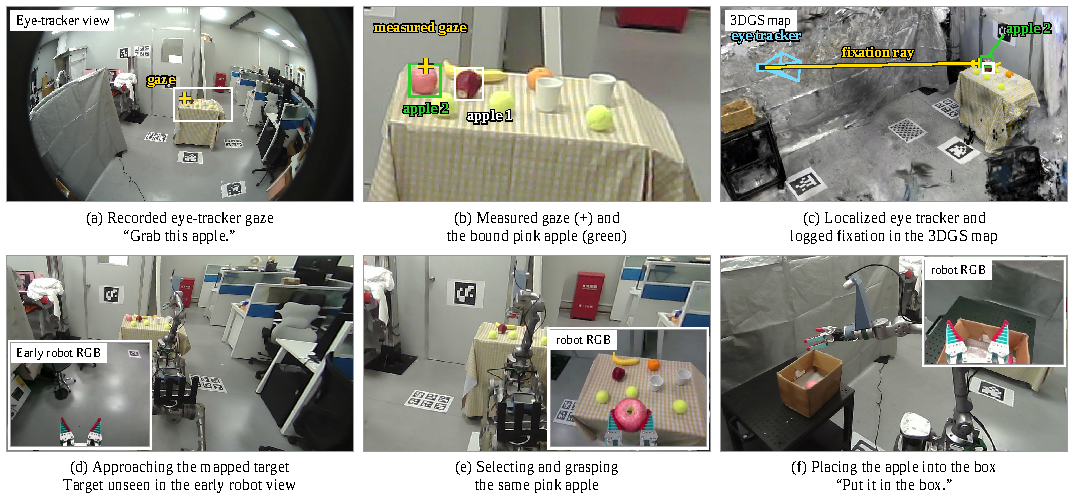
\includegraphics[width=\textwidth]{Figures/fig_story_pink_apple_icra.pdf}
  \caption{Gaze-guided instance selection across viewpoints.
  (a)--(b) The user looks toward the pink apple and says ``Grab this apple.''
  The recorded gaze resolves the request to apple 2 in the persistent 3DGS
  instance map. (c) The localized eye tracker and a logged fixation during
  the request are shown in the map. (d)--(e) The robot approaches the mapped
  target, observes the apples from a different viewpoint, and grasps the
  selected pink apple. (f) Following ``Put it in the box,'' the robot places
  it into the box. Yellow crosses indicate measured gaze; green outlines
  indicate the selected instance. The 2D markers use raw gaze near the
  displayed frame, while the 3D ray represents a calibrated, aggregated
  fixation. Robot RGB insets show the early approach with the target outside
  view, the grasped apple, and placement.}
  \label{fig:apple-cross-view}
\end{figure*}
